% =====================================================================
%  Four-page SPR manuscript: method, experiments, and discussion.
%  This version focuses on V1--V4 sampling stability and uses Lasso
%  as the estimator from the outset.
%  Figures: fig4p_forest_no_v5_en.pdf and fig4p_prediction_en.pdf.
% =====================================================================

\section{Method: Symmetric Preference Recovery}
\label{sec:method}

We first define investor behavior and the one-day-ahead forecasting task, and then construct
the state features and market context used to explain that behavior. We apply the same
conditional linear model to all three investor types and evaluate the sampling stability of
its coefficients through four validation procedures. We refer to this framework as
\emph{Symmetric Preference Recovery} (SPR). The recovered coefficients represent observed
conditional associations rather than structural preferences.

\subsection{Behavior Forecasting Problem}
\label{sec:setup}

Let $\mathcal I=\{\mathrm{foreign},\mathrm{institutional},\mathrm{individual}\}$ denote
the set of investor types. For investor type $i\in\mathcal I$ on trading day $t$, let
$V^{buy}_{i,t}$ and $V^{sell}_{i,t}$ be the total purchase and sale values. We define
normalized net-buying behavior as
\begin{equation}
u_{i,t}=\frac{V^{buy}_{i,t}-V^{sell}_{i,t}}{V^{buy}_{i,t}+V^{sell}_{i,t}}\in[-1,1]
\label{eq:action}
\end{equation}
This ratio scales net purchases by total trading value and preserves both direction and
intensity. The prediction target is $a_{i,t+1}=u_{i,t+1}$. The input state
$s_{i,t}=(x_{i,t},C_t)$ contains only information observed through day $t$.

All investor types share the same feature vector $x_{i,t}\in\mathbb R^3$, market context
$C_t\in\mathbb R^2$, and model specification; only the parameters are estimated separately.
Cross-type differences therefore reflect conditional responses learned along common
dimensions, rather than differences imposed by type-specific feature sets.

\subsection{State Features and Market Context}
\label{sec:features}

The state vector
$x_{i,t}=(x^{mom}_{t},x^{cross}_{i,t},x^{uw}_{i,t})^\top$ contains three features.

\textbf{Medium-term momentum.}
Let $P_t$ be the closing price of Samsung Electronics. We use the 20-day log return
\[
x^{mom}_{t}=\log(P_t/P_{t-20})
\]
with a prespecified horizon. A positive (negative) coefficient is consistent with
trend-following (contrarian) behavior~\cite{grinblatt2000investment,choe1999foreign}.

\textbf{Lagged cross-investor association.}
For the two types $j,k\ne i$, define
$x^{cross}_{i,t}=(u_{j,t-1}+u_{k,t-1})/2$. Using lagged behavior excludes the mechanical
offset among investor flows on the same trading day. This feature captures a lagged
cross-type relationship and is not a direct test of within-institution herding
~\cite{lakonishok1992impact}.

\textbf{Underwater position relative to average cost.}
Let $Q^b$ and $Q^s$ denote total purchase and sale quantities, and let $M^b$ and $M^s$
denote their corresponding values. The purchase VWAP is $P^b=M^b/Q^b$. In the following
recursion, we suppress the common indices $(i,t)$ and write $[v]_+=\max(v,0)$:
\begin{equation}
\begin{aligned}
\widetilde H&=\rho H_{t-1}, & H&=[\widetilde H+Q^b-Q^s]_+,\\
O&=[\widetilde H-Q^s]_+, & N&=H-O,\\
\bar P&=\frac{O\bar P_{t-1}+NP^b}{H},&
P^{vwap}&=\frac{M^b+M^s}{Q^b+Q^s}.
\end{aligned}
\label{eq:cost}
\end{equation}
Here, $\widetilde H$ is the decayed inventory carried into day $t$; $O$ is the portion of
old inventory remaining after sales; $N$ is newly retained inventory; and $H=O+N$ is total
effective inventory. The updated average cost is $\bar P$, while $P^{vwap}$ is the
same-day transaction VWAP. We initialize $H_{i,0}=0$ and omit zero-quantity terms from the
average-cost calculation. We define the underwater feature as
\[
x^{uw}_{i,t}=\left[(\bar P_{i,t}-P^{vwap}_{i,t})/\bar P_{i,t}\right]_+ .
\]
It is set to zero when effective inventory is zero or no trade occurs. The forgetting
factor $\rho=0.98$ gives
recent trades greater effective weight and implies a half-life of approximately 34 trading
days. This aggregate proxy may be sign-consistent with the disposition effect, but it is
not an account-level cost basis~\cite{shefrin1985disposition,odean1998investors}.

\textbf{Market context.}
Let $r_t$ be the one-day simple return on the KOSPI 200 and $e_t$ the closing KRW/USD
exchange rate. Define
$z^{FX}_t=(\log e_t-\mu_{t-1,252})/\sigma_{t-1,252}$, where
$\mu_{t-1,252}$ and $\sigma_{t-1,252}$ are the population mean and standard deviation of
$\{\log e_s:s=t-252,\ldots,t-1\}$. The ordered context vector is
$C_t=(r_t,z^{FX}_t)^\top$. All features and contexts are standardized using only the
training indices of each split. Feature-context correlations range from $-0.29$ to $0.22$;
we therefore interpret each coefficient as a conditional association holding the other
terms fixed.

\subsection{Conditional Behavior Model}
\label{sec:model}

For investor type $i$, the score describing next-day behavior is
\begin{equation}
q_{i,t}=(\beta_i+B_iC_t)^\top x_{i,t}+\alpha_i^\top C_t
\label{eq:model}
\end{equation}
where $\beta_i\in\mathbb R^3$ measures feature sensitivity in the average market context,
$B_i\in\mathbb R^{3\times2}$ captures context-dependent changes in that sensitivity, and
$\alpha_i\in\mathbb R^2$ captures the direct effect of the context when the features are
at their standardized means. Thus, $\beta_i+B_iC_t$ is the effective feature-weight vector
at time $t$.

Let $\mathrm{rvec}$ denote row-wise vectorization and define
\[
w_{i,t}=[x_{i,t};\mathrm{rvec}(x_{i,t}C_t^\top);C_t],\qquad
\theta_i=[\beta_i;\mathrm{rvec}(B_i);\alpha_i]
\]
so that $q_{i,t}=\theta_i^\top w_{i,t}$ and $\theta_i\in\mathbb R^{11}$. The predicted
behavior is $\hat a_{i,t+1}=\mathrm{clip}(\hat\theta_i^\top w_{i,t},-1,1)$.

\subsection{Estimation and Stability Validation}
\label{sec:protocol}

Let $\mathcal D_i$ denote the training indices for investor type $i$. We estimate the
coefficients by $L_1$-penalized least squares:
\begin{equation}
\hat\theta_i=\operatorname*{arg\,min}_{\theta}\ \Bigl\{\tfrac{1}{|\mathcal{D}_i|}
\!\!\sum_{t\in\mathcal{D}_i}\!\!\bigl(w_{i,t}^{\top}\theta-a_{i,t+1}\bigr)^{2}
+\lambda_i\lVert\theta\rVert_1\Bigr\}
\label{eq:loss}
\end{equation}
{\emergencystretch=1em
$\lambda_i\ge0$ is the type-specific penalty strength. The objective in
Eq.~\eqref{eq:loss} is convex, and coordinate descent obtains a global solution. To verify
uniqueness, define $n_i=|\mathcal D_i|$,
$W_i=[w_{i,t}^{\top}]_{t\in\mathcal D_i}$,
$y_i=[a_{i,t+1}]_{t\in\mathcal D_i}$. For $\lambda_i=0$, we verify that
$\mathrm{rank}(W_i)=11$. For $\lambda_i>0$, define the KKT vector
$g_i=2W_i^\top(y_i-W_i\hat\theta_i)/n_i$ and set
$E_i=\{j:|g_{i,j}|=\lambda_i\}$. We then verify
$\mathrm{rank}(W_{i,E_i})=|E_i|$. The solution is unique for all three investor types
in all 45 splits, with a worst-case condition number of 6.86.
}

Rather than interpreting a single fitted coefficient vector, we evaluate sampling stability
through four procedures.

\textbf{(V1) Combinatorial purged cross-validation.}
We construct 45 CPCV splits~\cite{lopez2018advances} by selecting two of ten chronological
folds for testing. We apply a one-day purge and a five-day embargo, and
fit every standardization step using training indices only. Because the splits share
observations, sign consistency is treated as a stability measure rather than a $p$-value.

\textbf{(V2) Calendar-month block bootstrap.}
To address this dependence, we resample calendar-month blocks with replacement 1{,}000 times
and construct 95\% confidence intervals. Monthly blocks preserve within-block serial
dependence in daily investor flows.

\textbf{(V3) Expanding walk-forward evaluation.}
Because a CPCV test fold may precede some training folds, we also conduct ten expanding window
evaluations. Starting with 400 observations, each window applies a five-day purge, predicts
the next 60 trading days, and then expands the training sample by 60 observations.

\textbf{(V4) Penalty substitution.}
To verify that the results are not artifacts of the $L_1$ penalty, we re-estimate the model
using an $L_2$ penalty and no penalty, and compare coefficient signs across specifications.

{\emergencystretch=1em
The evaluation metrics are directional accuracy, the correlation between predicted and
realized behavior, MAE, and out-of-sample $R^2$. Directional accuracy is the proportion of
observations for which the predicted and realized signs agree; we set $\mathrm{sign}(0)=0$.
The baseline prediction
for out-of-sample $R^2$ is the mean behavior in the training sample of each split. Because
the dispersion of behavior differs across investor types, absolute MAE values are not used
to rank the types.
}

% =====================================================================
\section{Experiments}
\label{sec:experiments}

\subsection{Data}
\label{sec:data}

We use the latest 973 daily observations for Samsung Electronics (005930) for which the
252-day exchange-rate history, 20-day momentum, and next-day behavior can all be computed.
The state dates span January 6, 2022, to December 29, 2025. The single-stock design provides
a controlled setting that removes cross-stock fixed effects and liquidity differences,
thereby isolating heterogeneity across investor types.

Mean behavior is close to zero for all three types, but its standard deviation is 0.334 for
individual investors, 0.257 for foreign investors, and 0.125 for institutions. Their
first-order autocorrelations are 0.345, 0.401, and 0.149, respectively. Same-day behavior
is strongly negatively correlated across types (foreign-individual: $-0.772$;
institutional-individual: $-0.499$). The gap between the sum of net purchases by the three
types and the market total, which includes other corporations and other foreign entities,
averages KRW 14.4 billion per day, or 1.3\% of trading value. The type-specific values of
$\lambda$ are $0$, $0.01$, and $0.0003$. They were carried over from a preceding
specification rather than selected by nested cross-validation in the present specification.
Assigning 0, 0.0005, or 0.01 as a common penalty for all three types does not alter the sign
classifications reported below.

\subsection{Coefficient and Sampling Stability (V1--V4)}
\label{sec:stability}

\begin{figure*}[t]
  \centering
  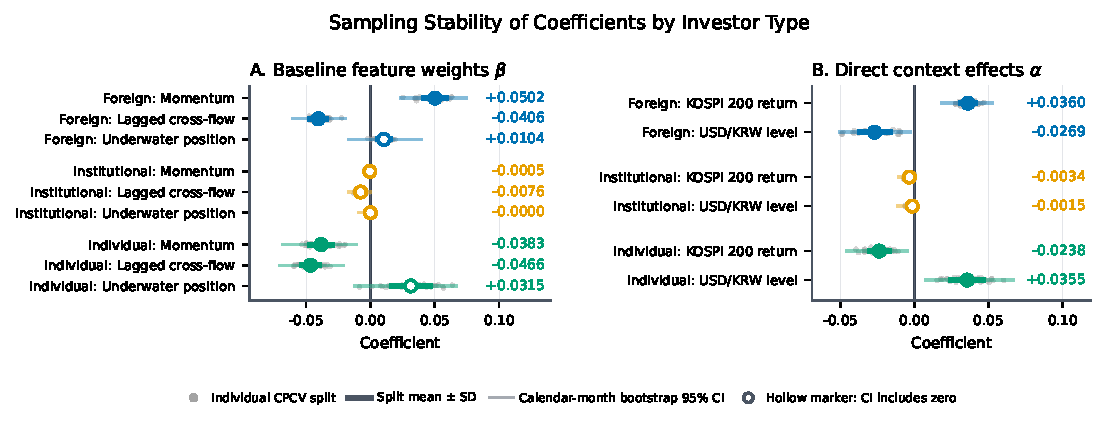
\includegraphics[width=\textwidth]{figures/fig4p_forest_no_v5_en.pdf}
  \caption{Sampling stability of the recovered coefficients. Gray dots denote the 45 CPCV
  splits, thick lines show the standard deviation across splits, and thin lines show
  calendar-month block-bootstrap 95\% confidence intervals. Hollow markers indicate
  intervals containing zero; values on the right are mean coefficients across splits.}
  \Description{A two-panel forest plot. The left panel displays momentum, lagged cross-flow,
  and underwater-position coefficients; the right panel displays the direct KOSPI 200 and
  exchange-rate effects for three investor types. The foreign and individual coefficients
  have opposite signs, while most institutional coefficients lie near zero.}
  \label{fig:forest}
\end{figure*}

\begin{table}[t]
  \caption{CPCV out-of-sample performance (mean $\pm$ standard deviation across 45 splits).
  The table checks that the model does not learn noise alone; it does not establish
  predictive superiority.}
  \label{tab:performance}
  \small
  \centering
  \begin{tabular}{@{}lccc@{}}
    \toprule
    Metric & Foreign & Institutional & Individual \\
    \midrule
    Directional accuracy & $0.636\pm0.040$ & $0.536\pm0.035$ & $0.602\pm0.044$ \\
    Correlation          & $0.279\pm0.106$ & $0.060\pm0.062$ & $0.239\pm0.116$ \\
    MAE                  & $0.195$ & $0.095$ & $0.266$ \\
    Out-of-sample $R^2$  & $0.105$ & $0.002$ & $0.102$ \\
    \bottomrule
  \end{tabular}
\end{table}

\begin{figure*}[t]
  \centering
  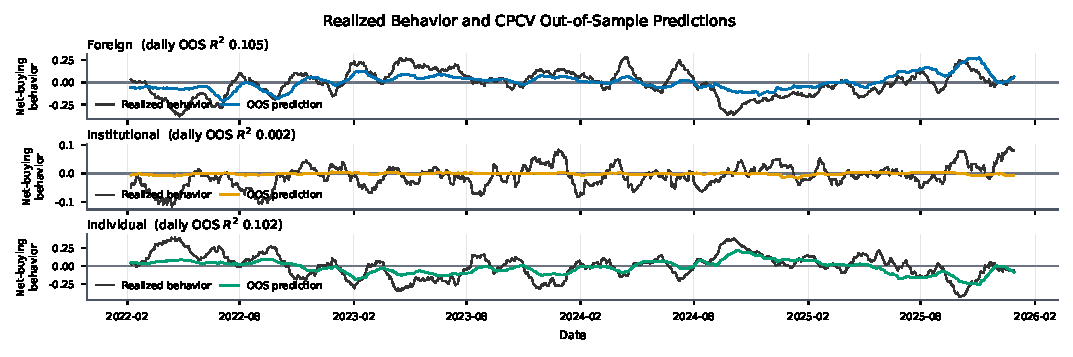
\includegraphics[width=\textwidth]{figures/fig4p_prediction_en.pdf}
  \caption{Realized behavior and CPCV out-of-sample predictions by investor type. We first
  average the nine CPCV test predictions available for each date and then apply a
  20-trading-day moving average to both realized and predicted behavior. Panel-level
  out-of-sample $R^2$ values are the 45-split means for unsmoothed daily predictions and
  match Table~\ref{tab:performance}.}
  \Description{Three time-series panels overlay realized net-buying behavior and
  out-of-sample predictions for foreign, institutional, and individual investors.
  Predictions track broad movements for foreign and individual investors, while the
  institutional prediction remains nearly flat around zero.}
  \label{fig:prediction}
\end{figure*}

The dispersion across splits in Table~\ref{tab:performance} precludes comparisons based on
any single split. In Figure~\ref{fig:prediction}, predictions for foreign and individual
investors follow broad trading-flow regimes, whereas institutional predictions remain near
zero. Coefficient stability shows the same contrast (Figure~\ref{fig:forest}).

\textbf{(V1)} The foreign momentum weight is $+0.0502$ and positive in all 45 splits,
whereas the individual weight is $-0.0383$ and negative in every split. Lagged cross-flow
coefficients are negative for all three types in every split. The individual underwater
coefficient is positive in 97.8\% of splits. For institutions, the Lasso sets momentum and
underwater coefficients exactly to zero in 36 and 44 of the 45 splits, respectively.

\textbf{(V2)} Eight coefficients have bootstrap intervals that exclude zero: momentum and
lagged cross-flow, together with both direct context effects, for foreign and individual
investors. The individual underwater interval ranges from $-0.0122$ to $+0.0665$, and all
institutional intervals include zero. Despite complete sign consistency across the 45 CPCV splits, the
individual underwater coefficient changes sign in 5.5\% of calendar-month resamples. This
result illustrates the warning in Section~\ref{sec:protocol}: because CPCV splits share
observations, sign consistency alone can understate uncertainty.

\textbf{(V3)} Expanding walk-forward performance varies considerably across windows.
Foreign directional accuracy is $0.610\pm0.116$, and its correlation is
$0.131\pm0.162$, less than half the CPCV correlation. We report this decline as a temporal
generalization limit. The coefficient paths are more stable. Foreign momentum remains
positive and individual momentum remains negative in all ten windows; the two paths never
cross. The same contrast holds for both direct context effects, while the institutional
paths remain near zero.

\textbf{(V4)} Foreign and individual coefficients agree to four decimal places under
$L_1$, $L_2$, and unpenalized estimation. Only institutional coefficients move with the
penalty; for example, lagged cross-flow changes from $-0.0076$ to $-0.0124$.

\textbf{Robustness.} Across the nine combinations of forgetting factors
$\rho\in\{0.95,0.98,0.99\}$ and momentum windows $\{10,20,60\}$, foreign and individual
momentum coefficients are positive and negative, respectively, in 100\% of specifications.
The individual underwater coefficient is positive in at least 91\%. Imposing a common
$\lambda$ across investor types leaves these sign classifications unchanged.

% =====================================================================
\section{Interpretation}
\label{sec:interpretation}

\begin{itemize}
\item \textbf{Foreign investors: stable conditional associations with market direction
and the exchange-rate regime.} The momentum weight of $+0.0502$ is positive in all
45 CPCV splits, and its calendar-month bootstrap interval excludes zero. The association
between recent price increases and greater foreign net buying is therefore insensitive to
the split and resampling scheme. The KOSPI 200 effect of $+0.0360$ and the exchange-rate
effect of $-0.0269$ pass the same checks. Conditional on the other features, foreign
investors tend to buy on market up-days and sell when the KRW is weak relative to the
preceding 252 days. These signs accord with prior evidence on foreign trend trading
~\cite{grinblatt2000investment,choe1999foreign}. The design does not separate counterparty
flows from common market shocks, so these patterns do not identify an independent
structural preference. For the same reason, the stable negative lagged cross-flow
coefficient is not direct evidence of anti-herding or imitation across investor types.

\item \textbf{Individual investors: opposing market associations and limited loss
avoidance.} Individual momentum ($-0.0383$), the KOSPI 200 effect
($-0.0238$), and the exchange-rate effect ($+0.0355$) have signs opposite to their
foreign counterparts. They remain stable across CPCV splits, calendar-month resampling,
walk-forward evaluation, and penalty substitution. Individual investors thus tend to sell
after stock and market increases and to buy during KRW-weakness regimes. The strong negative
same-day correlation between foreign and individual flows prevents this contrast from
identifying an independent individual contrarian preference. The underwater weight is
$+0.0315$ and positive in 97.8\% of CPCV splits and at least 91\% of robustness
specifications. A deeper loss relative to average cost is therefore associated with greater
net buying or reduced selling, a sign consistent with avoiding loss realization or averaging
down. However, the calendar-month interval includes zero, and aggregate flows cannot
distinguish additional purchases from deferred sales. We interpret the coefficient as a
limited, repeatedly observed signal rather than direct evidence of loss aversion.

\item \textbf{Institutions: no common behavioral weight in aggregate flows.} The data do
not reveal which information individual institutions use. Within the aggregate Korean
``institutional'' category, however, the specified features do not form a stable common
trading rule. The instability of all main coefficients and an out-of-sample $R^2$ of 0.002
are consistent with heterogeneous institutional responses offsetting one another during
aggregation.
\end{itemize}

\textbf{Synthesis.} Foreign and individual momentum, market, and exchange rate coefficients
point in opposite directions and remain stable across sample constructions. Individual
underwater positions retain a limited signal consistent with avoidance of loss realization,
whereas aggregate institutional flows reveal no common behavioral rule. The central result
is that these differences recur under a symmetric estimation design and four stability
checks. Decomposing their origins into independent preferences, counterparty absorption,
and common shocks lies outside the identification scope of the analysis.

% =====================================================================
\section{Limitations and Future Research}
\label{sec:limitations}

\textbf{(1) Interpretive scope.} The recovered weights are conditional associations rather
than causal effects. The model does not include returns, Sharpe ratios, or transaction costs;
Table~\ref{tab:performance} therefore does not establish the superiority of a trading rule
or flow forecast. Because the design does not separately identify the accounting offset in
same-day flows and common market shocks, the opposing foreign and individual coefficients
and the negative lagged cross-flow coefficients cannot be interpreted as independent
preferences.

\textbf{(2) Disposition-effect proxy.} The individual underwater coefficient does not pass
the calendar-month block bootstrap. Moreover, the average cost is an approximation based on
aggregate trades rather than realized gains and losses at the account level. Its sign is
consistent with the disposition effect, but it does not constitute a direct test.

\textbf{(3) Generalizability.} The single-stock setting controls for cross-stock
heterogeneity but has not been validated across other securities or markets.

\textbf{Future research.} First, applying the same estimator and V1--V4 procedures to
stocks with different foreign ownership and liquidity would test cross-sectional
generalizability. Second, distinguishing the accounting offset in simultaneous flows from
each investor type's direct response requires richer data or an alternative identification
design. Third, the hypothesis that aggregation produces institutional instability can be
tested directly by applying symmetric estimation to the KRX's disaggregated investor
categories.
